% kuleuventheme2 by Janez Kren, September 2017, janez.kren@kuleuven.be, based on:
% kuleuventheme 1.3 by Roland Pastorino, 2013 roland.pastorino@kuleuven.be / www.rolandpastorino.com

\PassOptionsToPackage{usenames, table, dvipsnames}{xcolor} % 
\documentclass[11pt,t]{beamer}
\usetheme{kuleuven2}	%THEME OPTIONS for LOGO: kul (default), kulak, lrd,    ; OPTIONS for TITLE PAGE: normal (default), sedes


%%% OTHER SETTINGS
\usefonttheme[onlymath]{serif}			% math font with serifs, delete to make it sans-serif
\setbeamertemplate{footline}[body] 		% delete this line to remove footline bar on all frames
%\usepackage[orientation=landscape,size=custom,width=16,height=9,scale=0.5,debug]{beamerposter} %enable for widescreen 16:9 ratio
%\titlegraphic{ \includegraphics[width=.2\paperwidth]{mytitlepagepic.png} } %optional title page image


%%% ADDED BY ALEX (start)
\usepackage[english]{babel}
\usepackage{amsfonts}
\usepackage{amssymb}

\usepackage{pythonhighlight}

\usepackage[orientation=landscape,size=custom, width=16,height=9,scale=0.5,debug]{beamerposter} 

\definecolor{mygray}{rgb}{0.8,0.8,0.8}
\newcommand{\inline}[1]{ \colorbox{mygray}{\lstinline{#1}}}

\usepackage{xcolor}

\usepackage{layouts} % To get text/page width

\usepackage{listings}
\definecolor{codegreen}{rgb}{0,0.6,0}
\definecolor{codegray}{rgb}{0.5,0.5,0.5}
\definecolor{codepurple}{rgb}{0.58,0,0.82}
% \definecolor{backcolour}{rgb}{0.95,0.95,0.92}
\definecolor{backcolour}{rgb}{0.93,0.93,0.95}
\lstdefinestyle{mystyle}{
    backgroundcolor=\color{backcolour},   
    commentstyle=\color{codegreen},
    keywordstyle=\color{magenta},
    numberstyle=\tiny\color{codegray},
    stringstyle=\color{codepurple},
    basicstyle=\ttfamily\footnotesize,
    breakatwhitespace=false,         
    breaklines=true,                 
    captionpos=b,                    
    keepspaces=true,                 
    numbers=left,                    
    numbersep=5pt,                  
    showspaces=false,                
    showstringspaces=false,
    showtabs=false,                  
    tabsize=2
}
\lstset{style=mystyle}

\usepackage{mathtools}
\DeclarePairedDelimiter\ceil{\lceil}{\rceil}

\usepackage{listings}

%%% Less vertical spacing in ToC
\makeatletter
\patchcmd{\beamer@sectionintoc}{\vskip1.5em}{\vskip0.75em}{}{}
\makeatother

%%% ADDED BY ALEX (stop)


%%% TITLE PAGE INFO:
\title[Geavanceerde Computerarchitectuur 4$^{\text{th}}$ Session]{Geavanceerde Computerarchitectuur 4$^{\text{th}}$ Session} %[]] will appear in footline
\subtitle{Optimization techniques, \\ Coalesced memory access and device (GPU) memory types}

\author{Thomas Feys, {\footnotesize thomas.feys@kueluven.be}}
\institute{DRAMCO -- WaveCore -- ESAT}
\date{Academic year 2024/25}


% Some resources
% https://nichijou.co/cuda5-coalesce/
% https://www.ce.jhu.edu/dalrymple/classes/602/Class13.pdf
% https://leimao.github.io/blog/CUDA-Constant-Memory/


\begin{document}
\csname beamer@calculateheadfoot\endcsname %recalculate head and foot dimension


 %%
 %%  0. TITLE PAGE and TABLE OF CONTENT
 %%
% Title page
\begin{frame}[plain,noframenumbering]
	\titlepage
\end{frame}
	

% Table of Contents
\begin{frame}{Outline}
	\hfill	{\large \parbox{.961\textwidth}{\vspace{4mm}\tableofcontents[hideothersubsections]}}
\end{frame}



\section{Intermezzo}

\begin{frame}[fragile]{Free allocated memory}

\begin{lstlisting}[language=C++]
#define SIZE 16
...
int* p1 = (int*)malloc(SIZE*sizeof(int));
int* p2;
cudaMalloc(&p2, SIZE*sizeof(int));
...
free(p1);
cudaFree(p2);
\end{lstlisting}

\vspace{4mm}

Otherwise memory leaks are introduced.

\vspace{2mm}

Can use \href{https://valgrind.org/}{Valgrind} to detect leaks.
    
\end{frame}


\section{GPU memory access and memory types}


\begin{frame}{Coalesced memory access}

    {\footnotesize \textit{Coalesce: to come together to form one larger group, substance, etc.}}

    \vspace{-2mm}
    
    \begin{columns}[t]
    \begin{column}{.5\textwidth}
        \vspace{0mm}
        \begin{itemize}\setlength\itemsep{0.75em}
            \item DRAM access is done in groups, typically 32, 64, or 128 bytes (high\nobreakdash-throughput parallel access)
            \item DRAM access is otherwise sequential (e.g. per request)
            \item Group memory access reduces memory latency
        \end{itemize}
    \end{column}
    \begin{column}{.52\textwidth}
    \vspace{-2mm}
        \begin{figure}
            \centering
            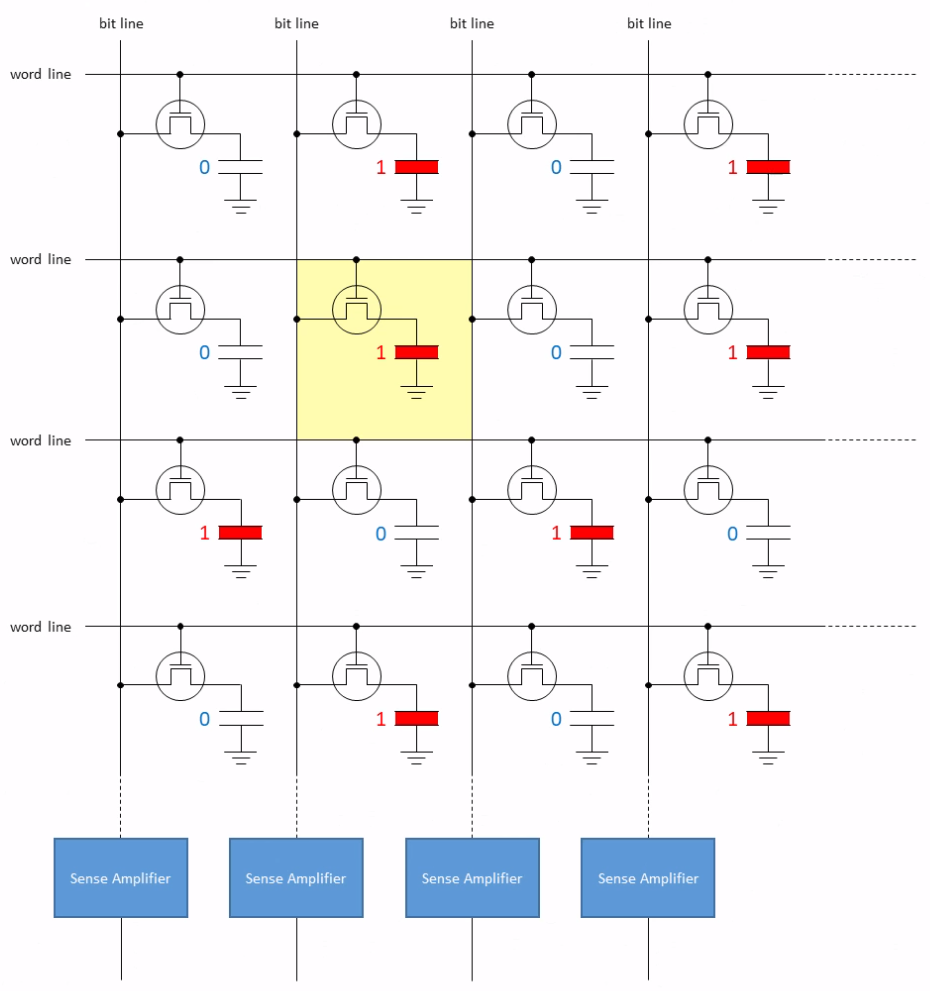
\includegraphics[width=0.7\columnwidth]{figure/session-4/dram.png}
        \end{figure}
    \end{column}
    \end{columns}
    
\end{frame}


\begin{frame}{Coalesced memory access}
    \begin{itemize}
        \item Is achieved when all threads in a warp access consecutive global memory locations.
        \item Threads in the same warp access global memory in a way that the hardware can combine (coalesce) their requests into as few memory transactions as possible.
        \item For example, for a given load instruction of a warp, if thread 0 accesses global memory location N, thread 1 location N+1, thread 2 location N+2, and so on, all these accesses will be coalesced into a as few memory requests as possible.
        \item Such coalesced access allows the DRAMs to deliver data as a burst.
    \end{itemize}
\end{frame}


\begin{frame}{Coalesced memory access in practice}

\begin{figure}
    \centering
    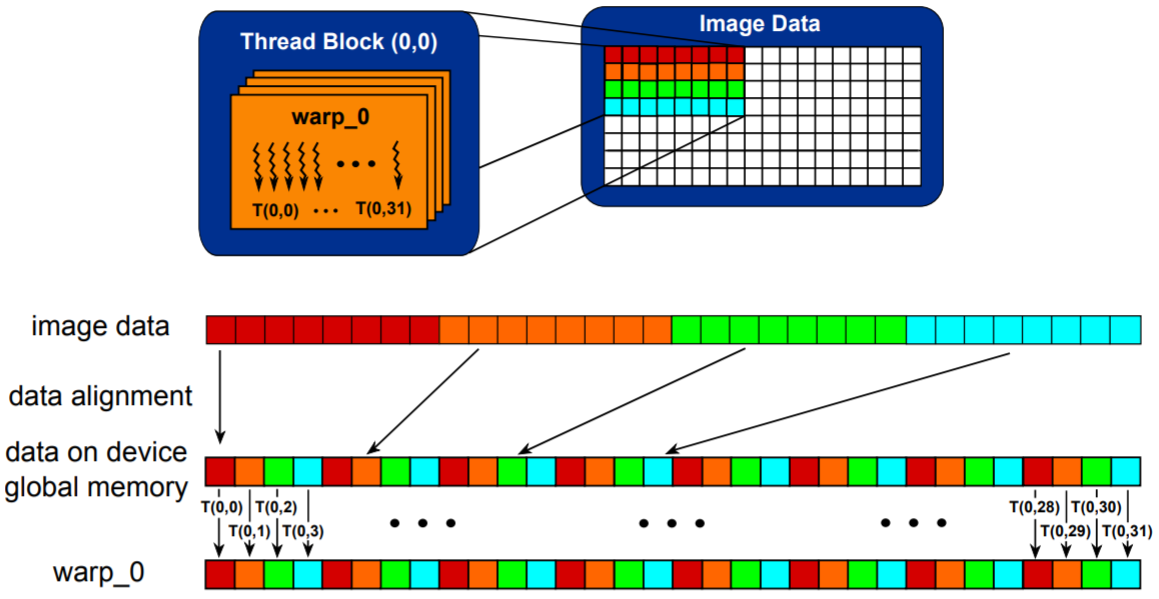
\includegraphics[width=0.7\columnwidth]{figure/session-4/coalesced.png}
\end{figure}

\end{frame}


\begin{frame}{Non-divergent threads and coalesced memory access}

\vspace{4mm}
\textbf{Non-divergent threads}

\vspace{4mm}
\noindent Threads in a \textbf{warp} take the same \textbf{computation} path (same complexity)
\vspace{10mm}

\textbf{Coalesced memory access}

\vspace{4mm}
\noindent Threads in a \textbf{warp} access the same \textbf{memory} group (adjacent addresses)

\end{frame}


\begin{frame}{GPU memory types}

    \begin{columns}[t]
    \begin{column}{.5\textwidth}
        \vspace{0mm}
        {\small
        \begin{itemize}\setlength\itemsep{0.75em}
            \item Shared -- Per block, on-chip
            \item Registers -- Per thread, on-chip
            \item Local -- Per thread, off-chip
            \item Constant -- For all, off-chip
            \item Global -- For all, off-chip
            \item Texture -- For all, off-chip
        \end{itemize}
        }
    \end{column}
    \begin{column}{.52\textwidth}
    \vspace{-4mm}
        \begin{figure}
            \centering
            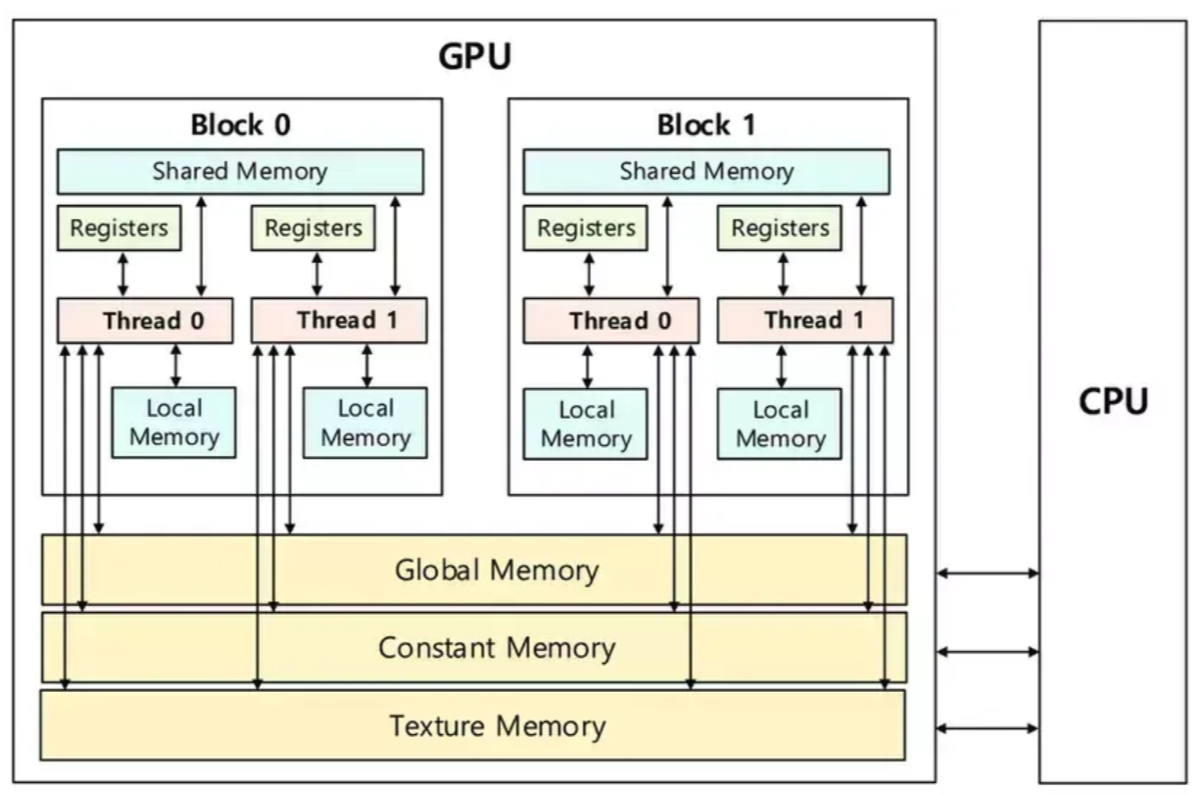
\includegraphics[width=1\columnwidth]{figure/session-4/memory_types.PNG}
        \end{figure}
    \end{column}
    \end{columns}
    
\end{frame}


\begin{frame}[fragile]{Global memory}

    \begin{itemize}
        \item Off-device -- high access latency
        \item All threads in the grid have access, as well as the CPU
        \item Large size -- typically several GB
        \item The 'default' option
    \end{itemize}
    
    \vspace{4mm}
    As in previous labs
\begin{lstlisting}[language=C++]
int* garr;
cudaMalloc(&garr, SIZE*sizeof(int));
// or (see analogy to constant memory in a later slide)
__device__ int garr[SIZE];
\end{lstlisting}
    
\end{frame}


\begin{frame}{Shared memory}

    \begin{itemize}
        \item On-device -- low access latency
        \item Shared among the threads of a single block
        \item User-managed cache, by default 48 kB (\inline{cudaFuncSetCacheConfig(...)})
        \item Two options in CUDA, see below
    \end{itemize}
    
    \vspace{4mm}
    Hardcode \inline{SIZE} (or use \inline{\#define}) \\
    \inline{my_kernel<<<blk, tpb>>>(...);} $\rightarrow$ \inline{__shared__ int smem[SIZE];}
    
    \vspace{4mm}
    Define size dynamically during kernel invocation \\
    \inline{my_kernel<<<blk, tpb, size>>>(...);} $\rightarrow$ \inline{extern __shared__ int smem[];}
    
\end{frame}


\begin{frame}{Workflow with shared memory}

    \emph{Threads migrate data from global to shared memory}
    \vspace{4mm}
    \begin{enumerate}\setlength\itemsep{0.75em}
        \item (on CPU) Copy data \textbf{to global memory} and run the kernel
        \item (on GPU, per thread) Migrate one or more elements \textbf{to shared memory}
        \item \textbf{Process} the data in \textbf{shared memory}
        \item Migrate the data \textbf{back to global memory}
        \item (on CPU) Copy data from global memory
    \end{enumerate}

    \vspace{4mm}
    \uncover<2->{Where should we put \inline{__syncthreads()}?}
    
\end{frame}


\begin{frame}[fragile]{Constant memory}

    \begin{itemize}\setlength\itemsep{0.25em}
        \item Off-device, optimized for low-latency read
        \item All threads in the grid have access, as well as the CPU
        \item Small size -- 64 KB
    \end{itemize}
    
    \vspace{4mm}
    From 
    \href{https://docs.nvidia.com/cuda/cuda-runtime-api/group__CUDART__MEMORY.html#group__CUDART__MEMORY_1g9bcf02b53644eee2bef9983d807084c7}{the documentation:}
\begin{lstlisting}[language=C++]
__constant__ int cmem[SIZE]; // GPU
...
int* arr; // CPU
...
cudaMemcpyToSymbol(cmem, arr, SIZE * sizeof(int)); // From CPU to GPU
\end{lstlisting}
    
\end{frame}


\begin{frame}{Other memory}

    \vspace{2mm}
    Registers
    {\footnotesize
    \begin{itemize}
        \item On-device -- Low access latency
        \item Access per thread
        \item \inline{threadIdx.x}
    \end{itemize}
    }
    
    \vspace{2mm}
    Local memory
    {\footnotesize
    \begin{itemize}
        \item Off-device -- High(er) access latency
        \item Access per thread
        \item \inline{int arr[128];}
    \end{itemize}
    }
    
    \vspace{2mm}
    Texture memory
    {\footnotesize
    \begin{itemize}
        \item Off-device with optimized read access
        \item Access for all threads
        \item For 2D graphic data
    \end{itemize}
    }
    
\end{frame}


\begin{frame}[fragile]{Regarding a question}

    \begin{figure}
        \centering
        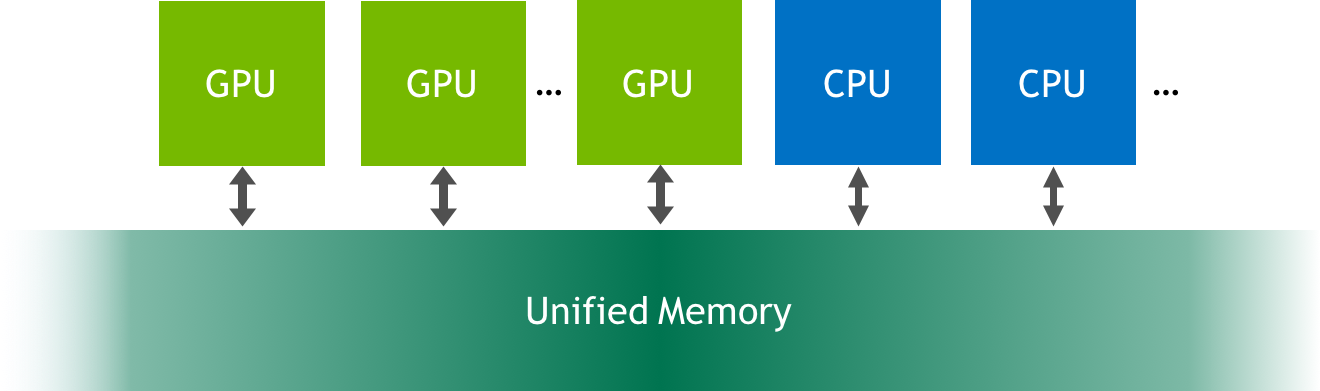
\includegraphics[width=0.8\linewidth]{figure/session-4/unified_memory.png}
    \end{figure}

    \vspace{2mm}
    
    \textit{Unified memory} allows one to allocate once and use on both devices. (Abstraction that handles memory migration.)



    \vspace{2mm}
    
    More \href{https://docs.nvidia.com/cuda/cuda-runtime-api/group__CUDART__MEMORY.html#group__CUDART__MEMORY_1gd228014f19cc0975ebe3e0dd2af6dd1b}{in the docs} and \href{https://developer.nvidia.com/blog/unified-memory-cuda-beginners/}{a blog post}.
    
\end{frame}


\section{Exercise}

\begin{frame}{Assignment}
Part 1 -- Coalesced memory access
\vspace{2mm}
\small{
\begin{itemize}\setlength\itemsep{0.75em}
    \item Design the following two kernels that operate on a square matrix $\mathbf{A}$ of size $N\times N$.
    \item Copy Kernel: $\mathbf{B} = \mathbf{A}$ (copy the input matrix to another matrix)
    \item Transpose Kernel: $\mathbf{B} = \mathbf{A}^T$ (transpose the input matrix)
    \item The matrix should be stored in \textbf{row-major order} as a contiguous 1D array (e.g., using \texttt{std::vector<float>}). 
    \item Element $\mathbf{A}[\text{row}][\text{col}]$ is stored at index: $\text{index} = \text{row} \times N + \text{col}$
    \item This memory layout affects both CPU cache performance and GPU memory coalescing %which is why transpose operations are often slower than copy operations.
    
\end{itemize}
}
\vspace{4mm}
\end{frame}

\begin{frame}{Assignment}
Part 1 -- Coalesced memory access
\vspace{2mm}
\small{
\begin{itemize}\setlength\itemsep{0.75em}
    \item Measure execution time.
    \item Compute effective bandwidth for each kernel ($BW = \frac{\text{Total bytes transferred}}{\mathrm{time}}$ in GB/s).
    \item Have a cpu implementation to verify the results and to compare the execution times.
    \item Repeat measurements to reduce noise and account for GPU warm-up effects.
    \item Observe how performance changes with matrix size and access pattern (which is faster and why?).
\end{itemize}
}
\vspace{4mm}
\end{frame}


\begin{frame}{Assignment}
Part 2 -- Global, shared, and constant memory
\vspace{2mm}
\begin{itemize}\setlength\itemsep{0.75em}
    \item Design a kernel that multiplies two matrices.
    \item Assess the processing time for a kernel that utilizes global\nobreakdash-only, global and shared, and global and constant memory.
\end{itemize}

\vspace{4mm}
\emph{Evaluations should consider changing the grid and/or input size.}
    
\end{frame}



\begin{frame}{Pointers -- Part 2}

    Recall matrix multiplication:
    
    \begin{figure}[t]
        \centering
        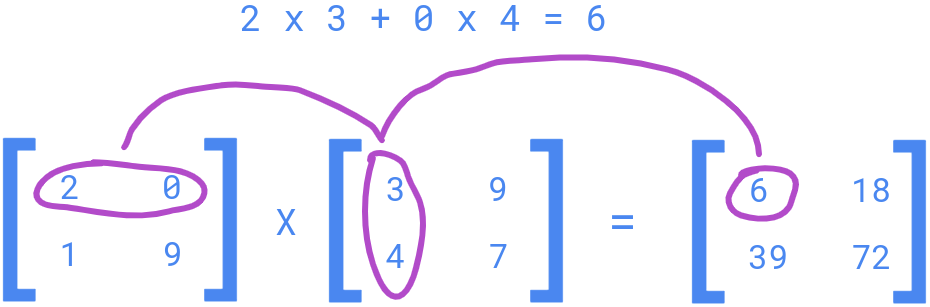
\includegraphics[width=0.8\columnwidth]{figure/session-4/matrix-multiplication.png}
    \end{figure}
    
    {\tiny Image source: \url{https://www.codingem.com/numpy-at-operator/}}

\end{frame}


\begin{frame}{Pointers -- Part 2}
\small{
    \begin{itemize}\setlength\itemsep{0.75em}
        \item Define an array that represents a matrix - in 1D or 2D form (start off with small square matrices and simple numbers for easier debugging).
        \item In this way define/allocate memory for three matrices, which will serve for $\mathbf{C} = \mathbf{AB}$.
        \item Make a kernel that uses only global memory to compute $\mathbf{C}$ $\rightarrow$ \textbf{verify the results}.
        \item Make a second and third matrix multiplication kernel, which use shared and constant memory, respectively, in addition to global memory.
        \item Time the kernels for different input and/or grid sizes. 
    \end{itemize}
}
\end{frame}


\begin{frame}{Guiding questions -- Part 2}
\small{
    \begin{itemize}\setlength\itemsep{0.75em}
        \item How much time does memory migration take (CPU to GPU global; GPU global to GPU shared)?
        \item How do the execution times of matrix multiplication compare when employing the three different memory types?
        \item How do the times scale with input and/or grid size?
    \end{itemize}
}
\end{frame}



\section{Appendix}


\begin{frame}[fragile]{Memory access during matrix multiplication} 
\label{naive_matmul}

\begin{columns}[t]
	\begin{column}{.45\textwidth}
	    \vspace{-2.0em}
        \begin{figure}[t]
            \centering
            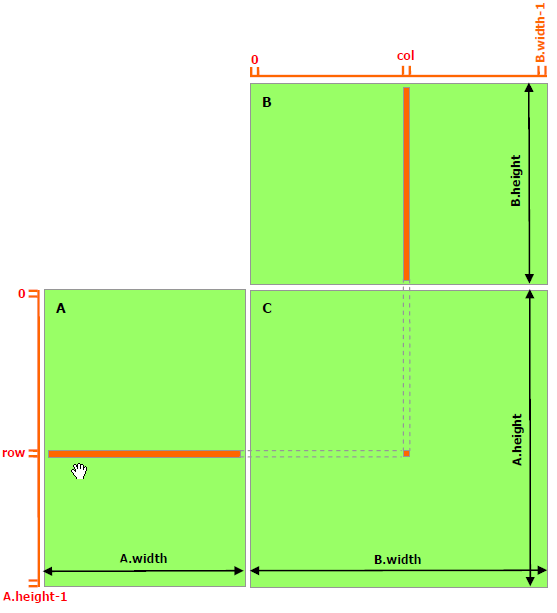
\includegraphics[width=0.95\columnwidth]{figure/session-4/matrix-multiplication-without-shared-memory.png}
        \end{figure}
	\end{column}
	\begin{column}{.55\textwidth} {\small
	    \vspace{-1.75em}
	    \begin{center}
	    \raggedright
	        Assume:
	        \vspace{0.1em}
    	    \begin{itemize} \setlength\itemsep{0.5 em}
    	        \item Matrices $\mathbf{A}$, $\mathbf{B}$, and $\mathbf{C}$ all NxN
    	        \item NxN grid of threads
    	    \end{itemize}
	        \vspace{0.5em}
	        Then:
	        \vspace{0.1em}
    	    \begin{itemize} \setlength\itemsep{0.5 em}
    	        \item Each thread writes 1 element in $\mathbf{C}$
    	        \item $\mathbf{A}$-rows and $\mathbf{B}$-columns are re-read N-1 times
    	    \end{itemize}
	    \end{center}
	    }
	\end{column}
\end{columns}
% ... discuss complexity on blackboard ...

\end{frame}



\begin{frame}[fragile]{Improvement by leveraging shared memory} 
\label{shared_memory_matmul}

\begin{columns}[t]
	\begin{column}{.45\textwidth}
	    \vspace{-2.0em}
        \begin{figure}[t]
            \centering
            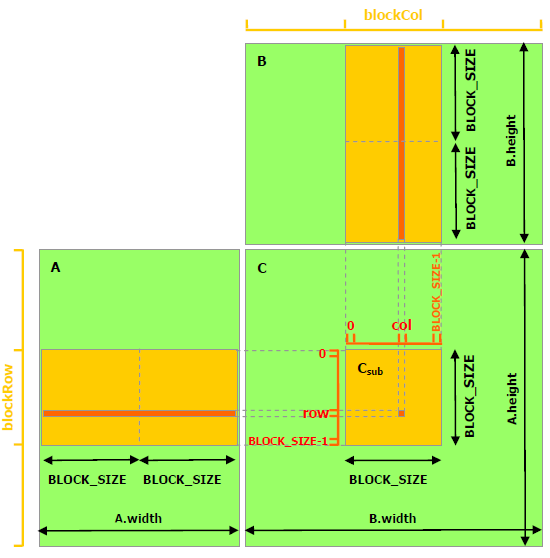
\includegraphics[width=\columnwidth]{figure/session-4/matrix-multiplication-with-shared-memory.png}
        \end{figure}
	\end{column}
	\begin{column}{.55\textwidth}{\small
	    \vspace{-1.75em}
	    \begin{center}
	    \raggedright
	        Assume:
	        \vspace{0.1em}
    	    \begin{itemize} \setlength\itemsep{0.5 em}
    	        \item Matrices $\mathbf{A}$, $\mathbf{B}$, and $\mathbf{C}$ all NxN
    	        \item NxN grid of threads
    	        \item Square blocks with size BLOCK\_SIZE
    	    \end{itemize}
	        \vspace{0.5em}
	        Then:
	        \vspace{0.1em}
    	    \begin{itemize} \setlength\itemsep{0.5 em}
    	        \item Each thread writes 1 element in $\mathbf{C}$
    	        \item Each thread copies one element from both $\mathbf{A}$ and $\mathbf{B}$ to shared memory, $k$-times
    	        \item $\mathbf{A}$-rows and $\mathbf{B}$-columns are re-read $k$-times
    	        \item $k = \frac{N}{BLOCK\_SIZE}$
    	    \end{itemize}
	    \end{center}
	    }
	\end{column}
\end{columns}
% ... discuss kernel design on blackboard ...

\end{frame}



\section{Sources}

\begin{frame}{Sources}

\begin{itemize}
    \item \href{https://www.oxfordlearnersdictionaries.com/definition/english/coalesce?q=coalesced}{Coalesced meaning} 
    \item \href{https://www.youtube.com/watch?app=desktop&v=I-9XWtdW_Co}{DRAM intro}
    \item \href{https://www.researchgate.net/publication/265849053_A_GPU_Accelerated_Algorithm_for_Blood_Detection_inWireless_Capsule_Endoscopy_Images}{Coalesced access figure}
    \item \href{https://developer.nvidia.com/blog/unified-memory-cuda-beginners/}{Blog post about unified access}
    \item \href{https://developer.nvidia.com/blog/using-shared-memory-cuda-cc/}{Blog post about shared memory}
    \item \href{https://giahuy04.medium.com/memory-types-in-gpu-6373b7a0ca47}{GPU memory figure}
\end{itemize}

\end{frame}


\end{document}
\fancyarrow{Hello}{World}.